\section{Quadrature Decomposition}
This suggestion is proposed to the decomposition method. Recall the recursive scheme (\ref{eq:recur_deco}) that was obtained in for approximating the solution; the idea of this experiment is based on the fact that the solution is approximated in terms of the Riemann-Liouville integral for an unspecified time $t$. This implies that the approximation is a function of $t$ and it could be approximated for each point on the partitioned interval $[0,T]$; this means that the Riemann-Liouville integral would no longer be a function of $t$ and it would rather be an standard definite integral, which can be approximated using classical quadrature rules (trapezoidal or Simpson rules).

In order to test the proposed scheme, we will use the following integer system or ODEs, and the results are shown in figure \ref{fig:qDeco_ex}.
\begin{equation}
  \begin{cases}
    x'=y&x(0)=1\\
    y'=2x-y&y(0)=-1
  \end{cases}
\end{equation}

Clearly, this approach did not give a correct approximation, not even for an integer-order system of ODEs. This is due to the fact that the classical quadrature formulas do not take information about the complete history of the function but only taking some points (not even taking information about the polynomial in the previous step), losing important information about the past of the function and it is unable to make an accurate approximation. 

¿TIENE SENTIDO? Es un ode... no importa la memoria, ¿o sí?

\begin{figure}[H]
  \centering
  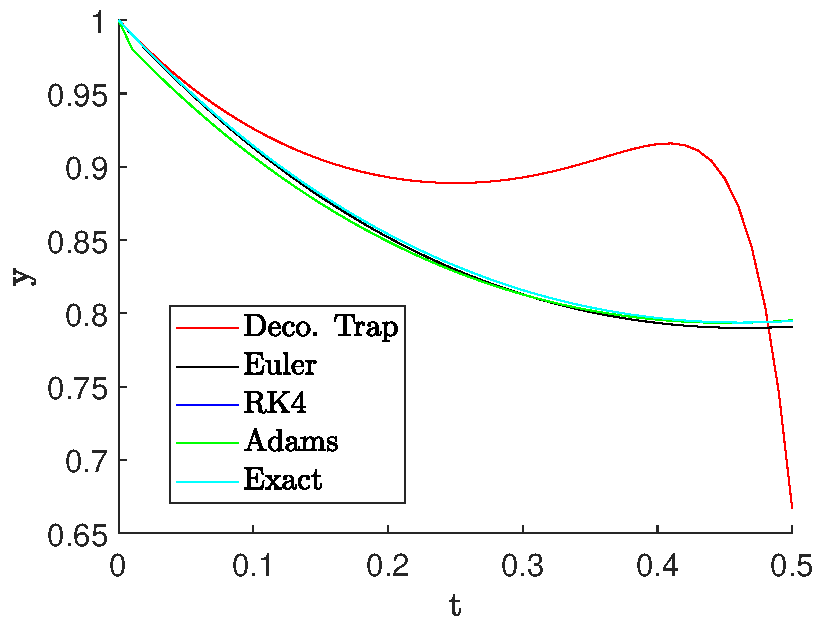
\includegraphics[scale=.5]{files/decom_trap.pdf}
  \caption{Results for quadrature decomposition.}
  \label{fig:qDeco_ex}
\end{figure}
